%%% Preamble
\documentclass[paper=a4, fontsize=11pt]{scrartcl}	% Article class of KOMA-script with 11pt font and a4 format

\usepackage[english]{babel}															% English language/hyphenation
\usepackage[protrusion=true,expansion=true]{microtype}				% Better typography
\usepackage{amsmath,amsfonts,amsthm}										% Math packages
\usepackage[pdftex]{graphicx}														% Enable pdflatex
%\usepackage{color,transparent}													% If you use color and/or transparency
\usepackage[hang, small,labelfont=bf,up,textfont=it,up]{caption}	% Custom captions under/above floats
\usepackage{epstopdf}																	% Converts .eps to .pdf
\usepackage{subfig}																		% Subfigures
\usepackage{booktabs}																	% Nicer tables
\usepackage{graphicx}
\graphicspath{ {images/} }

%%% Advanced verbatim environment
\usepackage{verbatim}
\usepackage{fancyvrb}
\DefineShortVerb{\|}								% delimiter to display inline verbatim text


%%% Custom sectioning (sectsty package)
\usepackage{sectsty}								% Custom sectioning (see below)
\allsectionsfont{%									% Change font of al section commands
	\usefont{OT1}{bch}{b}{n}%					% bch-b-n: CharterBT-Bold font
%	\hspace{15pt}%									% Uncomment for indentation
	}

\sectionfont{%										% Change font of \section command
	\usefont{OT1}{bch}{b}{n}%					% bch-b-n: CharterBT-Bold font
	\sectionrule{0pt}{0pt}{-5pt}{0.8pt}%	% Horizontal rule below section
	}


%%% Custom headers/footers (fancyhdr package)
\usepackage{fancyhdr}
\pagestyle{fancyplain}
\fancyhead{}														% No page header
\fancyfoot[C]{\thepage}										% Pagenumbering at center of footer
\fancyfoot[R]{\small \texttt{Victor Frolov}}	% You can remove/edit this line 
\renewcommand{\headrulewidth}{0pt}				% Remove header underlines
\renewcommand{\footrulewidth}{0pt}				% Remove footer underlines
\setlength{\headheight}{13.6pt}

%%% Equation and float numbering
\numberwithin{equation}{section}															% Equationnumbering: section.eq#
\numberwithin{figure}{section}																% Figurenumbering: section.fig#
\numberwithin{table}{section}																% Tablenumbering: section.tab#


%%% Title	
\title{ \vspace{-1in} 	\usefont{OT1}{bch}{b}{n}
		\huge \strut Battle of the Wearables and Their Interaction Designs \strut \\
		\Large \bfseries \strut Comparing the Apple Watch to Google Glass \strut
}
\author{ 									\usefont{OT1}{bch}{m}{n}
        Victor Frolov\\		\usefont{OT1}{bch}{m}{n}
        Loyola Marymount University\\	\usefont{OT1}{bch}{m}{n}
	Assignment 0924\\
}
\date{September 24, 2015}

%%% Begin document
\begin{document}
\maketitle
\section{Introduction}
	Wearable technology is becoming mainstream and is ranging from products such as fitness trackers, accessories to phones and even glasses that display information and allow you a virtual reality HUD. This report will attempt to objectively declare a superior user experience through interaction design from two infamous competing companies: Google and Apple.

	Below are two sections; the first provides usability measures and a conclusion on which device performed better, and the second dives into why this was the case. The usability of the  Apple Watch versus Google Glass will be measured with the following three tasks: 

\begin{itemize}
	\item Have the user send the following text message to any contact: ``I'm sorry Dave, I'm afraid I can't do that."
	\item Have the user set driving directions from Loyola Marymount University to Staples Center.
	\item Have the user set  a reminder for October 10th, 2017, with the title "Thanks Obama"
\end{itemize}

The measurable usabilities will fall under the following three categories: Learnability, Errors and Satisfaction.


\section{Usability Measures}
\subsection{Task One: Sending a text message}
The user must send the following text message to the contact \textit{Aleksandar Frolov} : ``I'm sorry Dave, I'm afraid I can't do that.''


\subsubsection{Learnability}

Users were timed, demonstrating how long it would take someone who has never used the device to complete a task. Each bar represents a user, and the height represents how many seconds it took to complete the task. It is obvious that the Apple Watch's learnability beat out Google Glass.

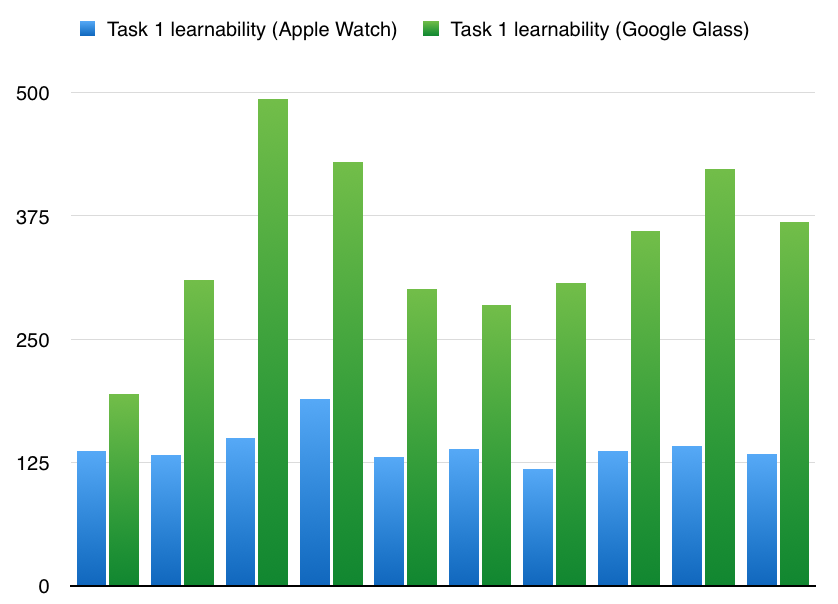
\includegraphics[scale=0.7]{charttask1}

Below is the average time for a user to complete a task, in seconds. Green bar's height represents the average time to complete the task using Google Glass in seconds, and the blue bar represents the average time to complete the task in seconds using the Apple Watch.

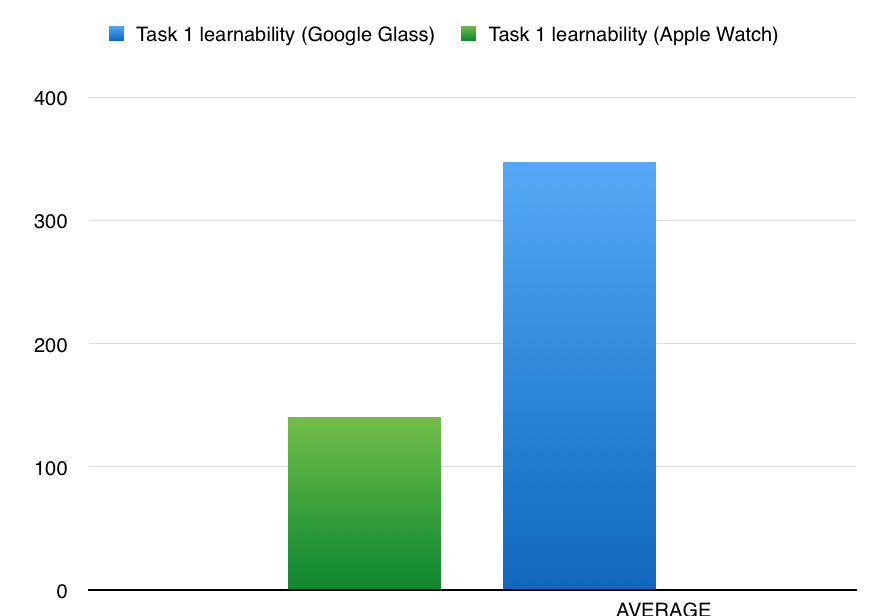
\includegraphics[scale=0.6]{task1average}

The Apple Watch's Average time to complete the task was 140.4 seconds, whereas Google Glass took 347, which was almost 2.5 times slower.


\subsubsection{Errors}
User errors were tracked when attempting to send a text message.

\textbf{Apple Watch}
4 out of 10 users assumed that pressing on crown would open keyboard and returned to the home screen instead. The same 4 users  shut off the screen by pressing lock button right after.
3 out of 10 users had voice recognition issues, which  may have been due to slurring of the words.
1 user was stuck in the watch face, confused how to exit it.


\textbf{Google Watch}
10 out of 10 users mistapped or swiped incorrectly causing the user to return back to the menu. 
6 out of 10 users had voice recognition issues, where the message would cut out early. Could be due to slurring of the words.


\subsubsection{Satisfaction}
Below is the user overall satisfaction when attempting to send the text message.

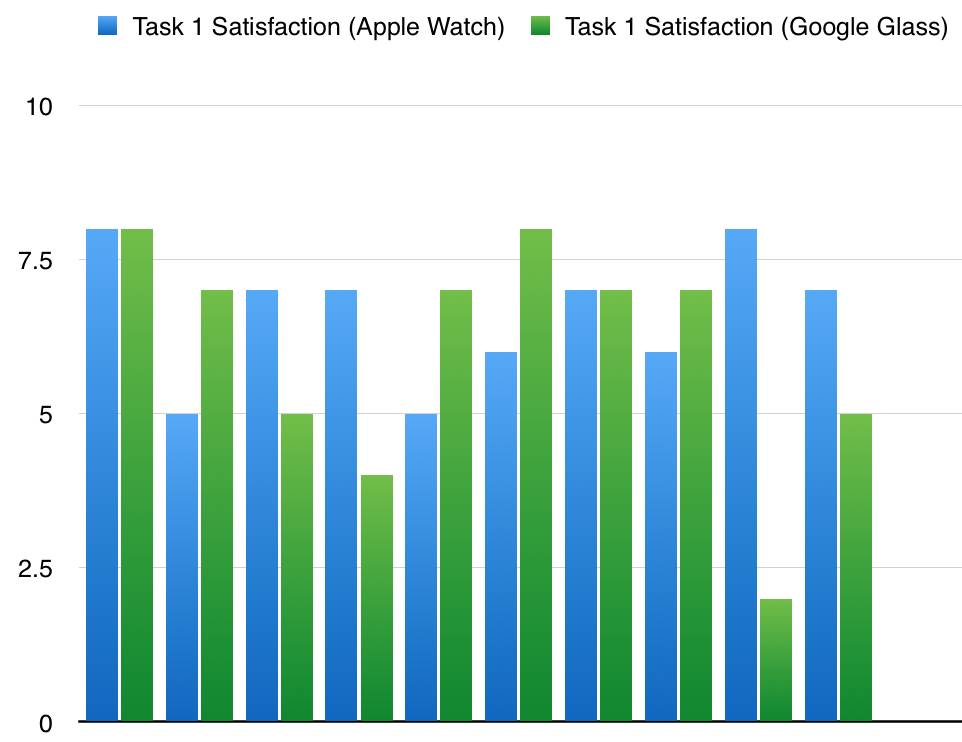
\includegraphics[scale=0.8]{task1satisfaction}\\ \\

Below is the average satisfaction (blue represents Apple Watch, green represents Google Glass)\\ \\

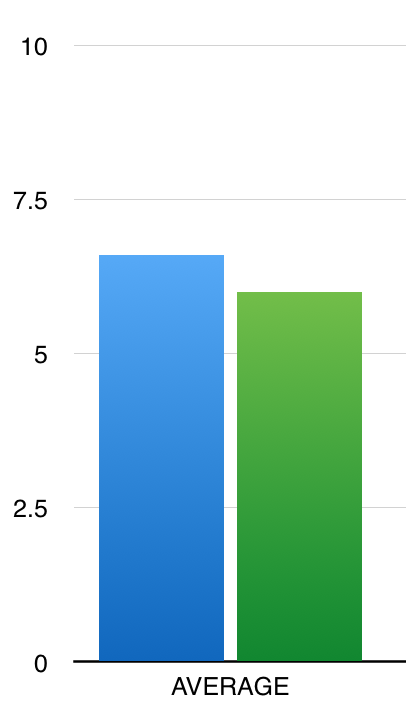
\includegraphics[scale=0.8]{task1satav}



Remarkably, even though each user struggled using Google Glass, and ran into far more errors, and took much longer on average to send a text message(with the only outlier being a quick completion) the subjective satisfaction was very close, landing at 6.6/10 for the Apple Watch, and 6/10 for Google Glass

\subsection{Task Two: Set Driving Directions}
Have the user set driving directions from Loyola Marymount University to Staples Center.

\subsubsection{Learnability}
Users were timed, demonstrating how long it would take someone who has never used the device to complete a task. Each bar represents a user, and the height represents how many seconds it took to complete the task. It is obvious that the Apple Watch's learnability beat out Google Glass.

Below is a chart for time taken to complete the task (each bar represents a user, and the time on the y axis is in seconds)

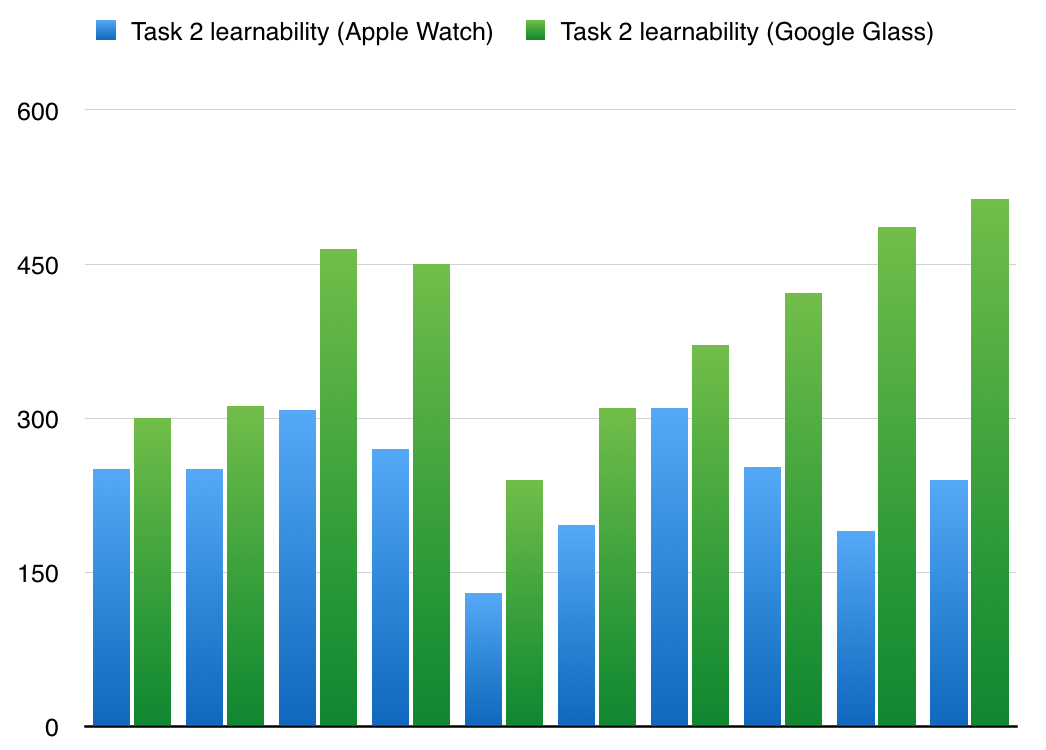
\includegraphics[scale=0.8]{task2learnability}


Below is a chart for time taken to complete the task on average, where the y axis is in seconds.

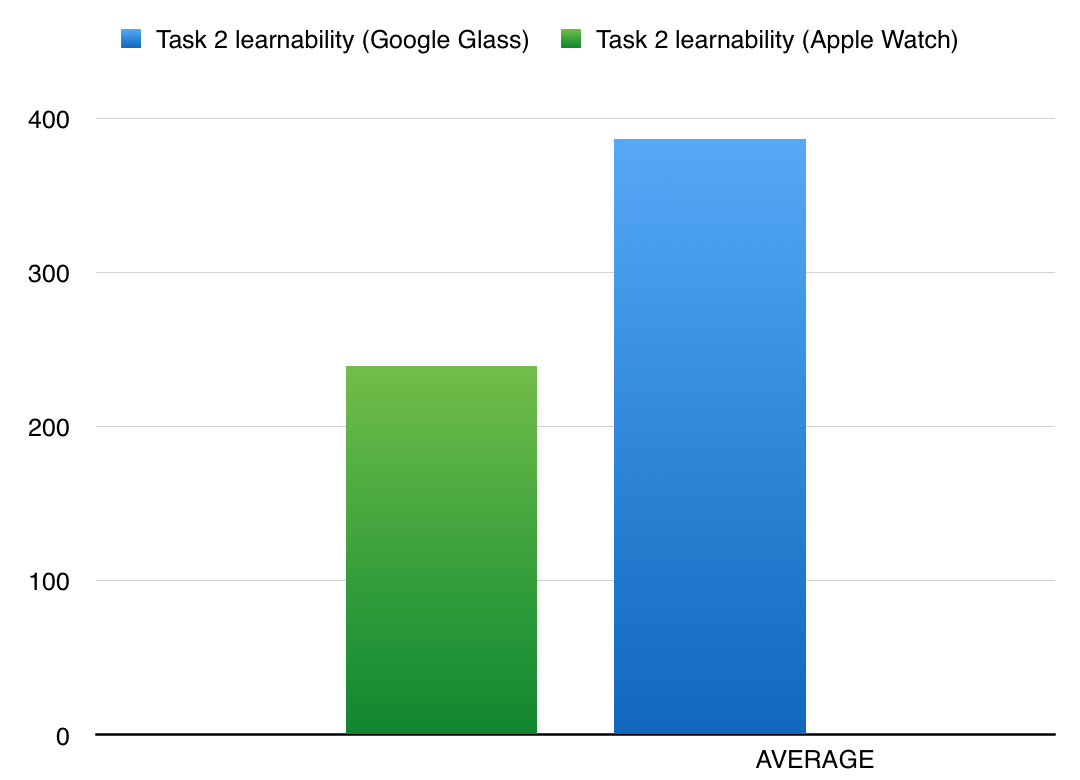
\includegraphics[scale=0.6]{task2learnav}

On average, users were 1.6 times faster on the Apple Watch than they were on Google Glass. Comparing to task 1, this is much closer.

\subsubsection{Errors}

User errors were tracked when attempting to navigate.\\

\textbf{Apple Watch} \\
9 out of 10 users pressed on crown assuming it would drop a pin. 4/10 attempted pinch to zoom functionality, and were unsucessful.

\textbf{Google Watch}\\
4 out of 10 users mistapped causing the app to quit. 3 out of 10 users were impatient and continued to tap on the touch pad due to map loading slowly. 5 out of 10 users found it unintuitive to drop a pin, and found that the most difficult part (while located at LMU). 2 out of 10 users got directions to Staples instead of the Staples Center.


\subsubsection{Satisfaction}
Below is the user overall satisfaction when attempting to find directions.

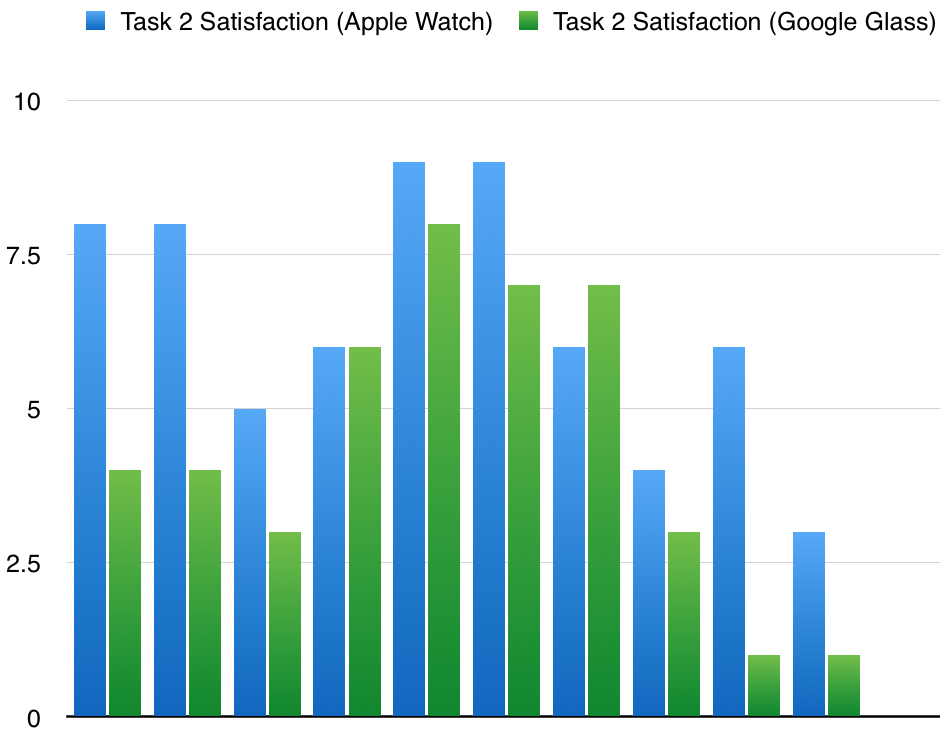
\includegraphics[scale=0.8]{task2sat}\\ \\

Below is the average satisfaction (blue represents Apple Watch, green represents Google Glass)\\ \\

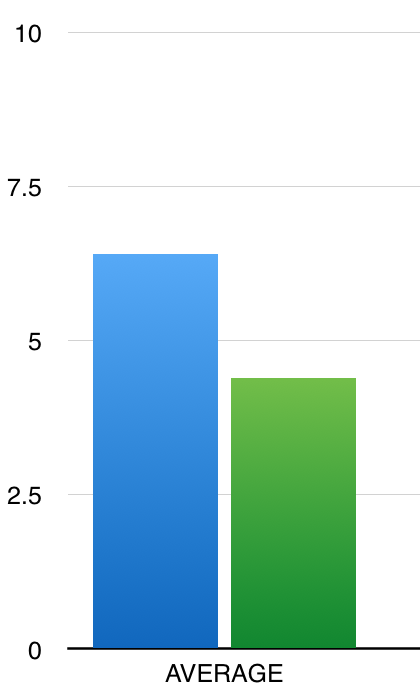
\includegraphics[scale=0.8]{task2satav}

Average for satisfaction for the Apple Watch and Google Glass were 6.4/10 and 4.4/10 respectively. Albeit being relatively close, the Google Glass got very unfavorable reviews, only one user graded satisfaction above a 7, while three users satisfaction above a 7 for Apple Watch.

\subsection{Task Three: Set Reminder}
Have the user set  a reminder for October 10th, 2017, with the title "Thanks Obama"

\subsubsection{Learnability}
Users were timed, demonstrating how long it would take someone who has never used the device to complete a task. Each bar represents a user, and the height represents how many seconds it took to complete the task. 

Below is a chart for time taken to complete the task (each bar represents a user, and the time on the y axis is in seconds)

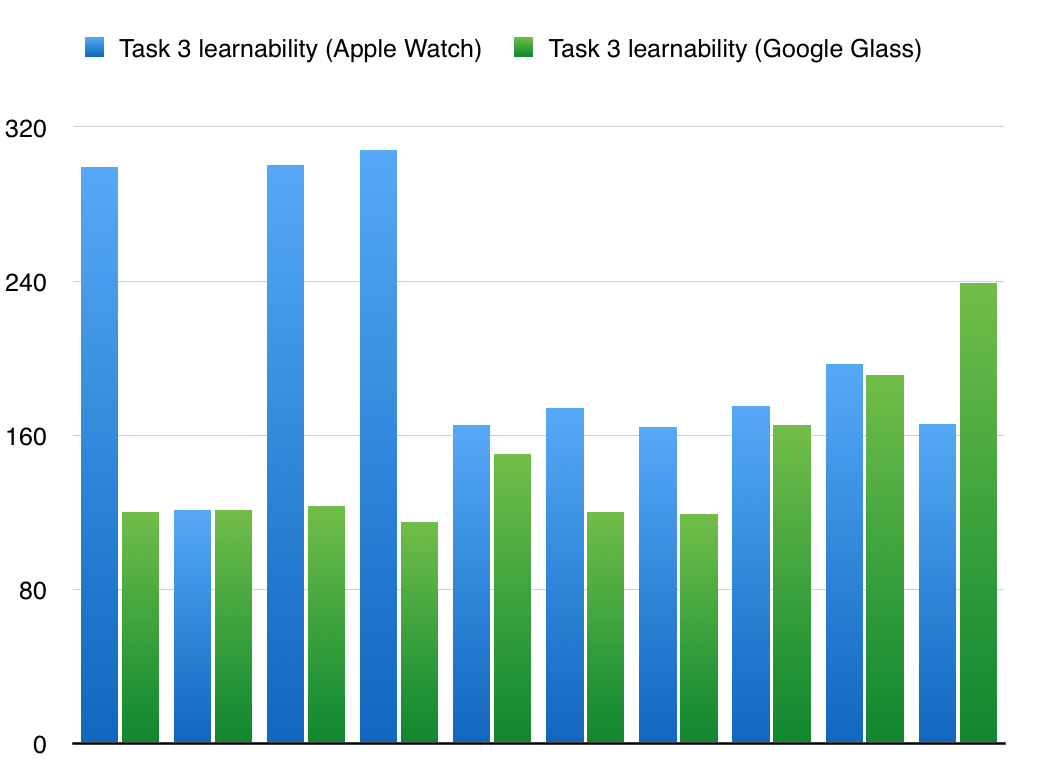
\includegraphics[scale=0.8]{task3learnability}


Below is a chart for time taken to complete the task on average, where the y axis is in seconds.

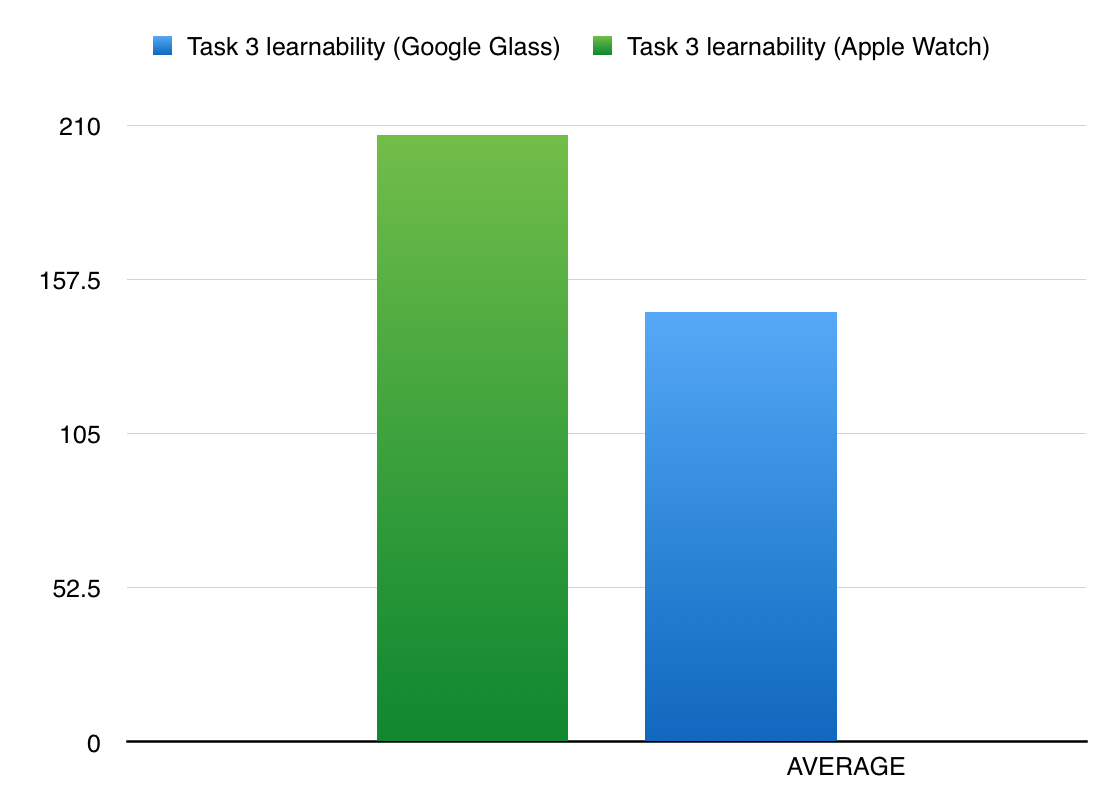
\includegraphics[scale=0.6]{task3learnav}

On average users were 1.4 times faster in completing the reminders task on Google Glass over Apple Watch, with 206.9 seconds average for the watch, and 146.3 seconds average for the glasses. This is the only one of the three tasks where users completed a task faster on Google Glass than on the Apple Watch.


\subsubsection{Errors}
User errors were tracked when attempting to set a reminder.\\

\textbf{Apple Watch} \\
2 out of 10 users accidentally quit the application, having to restart from scratch(action to quit application was not provided by tester). 3 out10 users encountered voice command issues, could be slurring of the words. 3 out of 10 users put the incorrect date having to restart from scratch.
 
\textbf{Google Watch}\\
Remarkably, there were no errors for any users.

\subsubsection{Satisfaction}
Below is the user overall satisfaction when attempting to set a reminder.

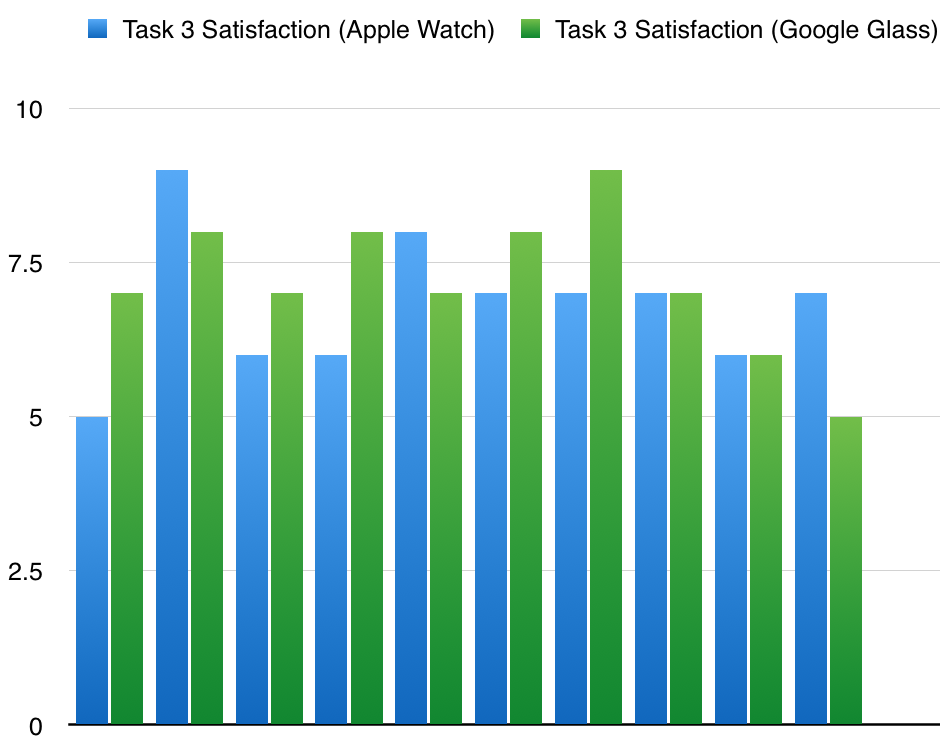
\includegraphics[scale=0.8]{task3sat}\\ \\

Below is the average satisfaction (blue represents Apple Watch, green represents Google Glass)\\ \\

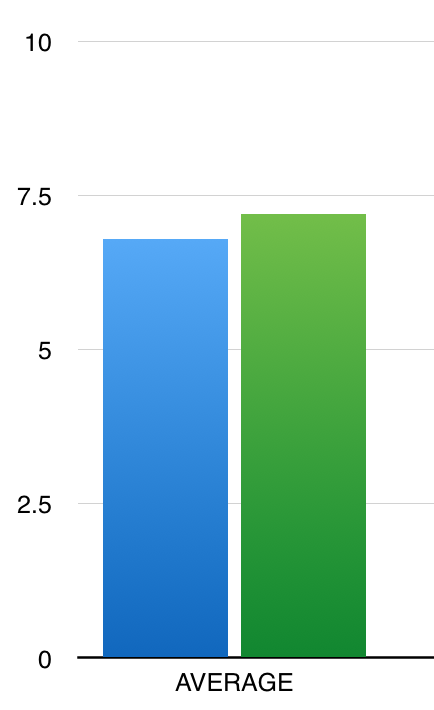
\includegraphics[scale=0.8]{task3satav}

Average for satisfaction for the Apple Watch and Google Glass were 6.8/10 and 7.2/10 respectively. Albeit the Apple Watch taking considerably longer (1 min), the user experience was almost identical.




\subsubsection{Conclusion}
Deciding on which of the two wearables has better interaction design is a hard question to answer. There are many factors to take into consideration. For example, people are relatively familiar with touch screens, and the apple watch is simply a smaller touch screen with force touch, but a product like Google Glass is something most people have never experienced. Another consideration to have is the Apple Watch being a finalized product sold to end users, whereas Google Glass was still under beta prior to it being shut down.  

Regardless, we have measurable statistics above to come to a conclusion, so to summarize, the Apple watch was considerably faster to accomplish all three tasks, averaging at 199 seconds, whereas Google Glass averaged at 291. User errors were all over the place, but all 10 out of 10 users mistapped on Google Glass in the first task. User satisfaction averaged a 6.6 for the Apple Watch, and 5.9 for Google Glass, so it appears that the Apple Watch performed better. 



\section{Explanations}
The most interesting aspect of evaluating the Apple Watch and Google Glass is that one was a finalized fully fleshed out device that had predecessors such as pebble and many android watches, while the other was first of it's kind, and was discontinued before being made available to the masses. Both devices try to serve the same purpose: allow the user to interact less with technology while going about their day. These devices don't want the user  to waste his time pulling out a phones if they get a notification or an email, and tread through their days with little to no slow-down. The biggest barrier of entry for both the Apple Watch and Google Glass are their respective mental models, and how intuitively the end user will adapt to them. \par

Watches historically serve three purposes: telling a user the time, adding style through accessories, and act as a status symbol. Apple made sure to make the Apple Watch be incredibly customizable, recently releasing countless setups to attract any style, ranging from rich CEO's that want a more conservative classic style, to runners who want durable and comfortable wearables, and everything in between. On the status symbol side, they made sure to release a Gold edition that costs up to  \$17,000. A steep price to pay for a device that will become outdated after just a year or two.\par

The Apple Watch had a genius implementation of something everyone is aware of: a crown on a watch. We are so used to seeing this on a watch and know it has functionality, that it is very intuitive to use. Dubbing it the "Digital Crown", users can center their view and relocate to the apps menu. It acts somewhat like the Home button on the iPhone.

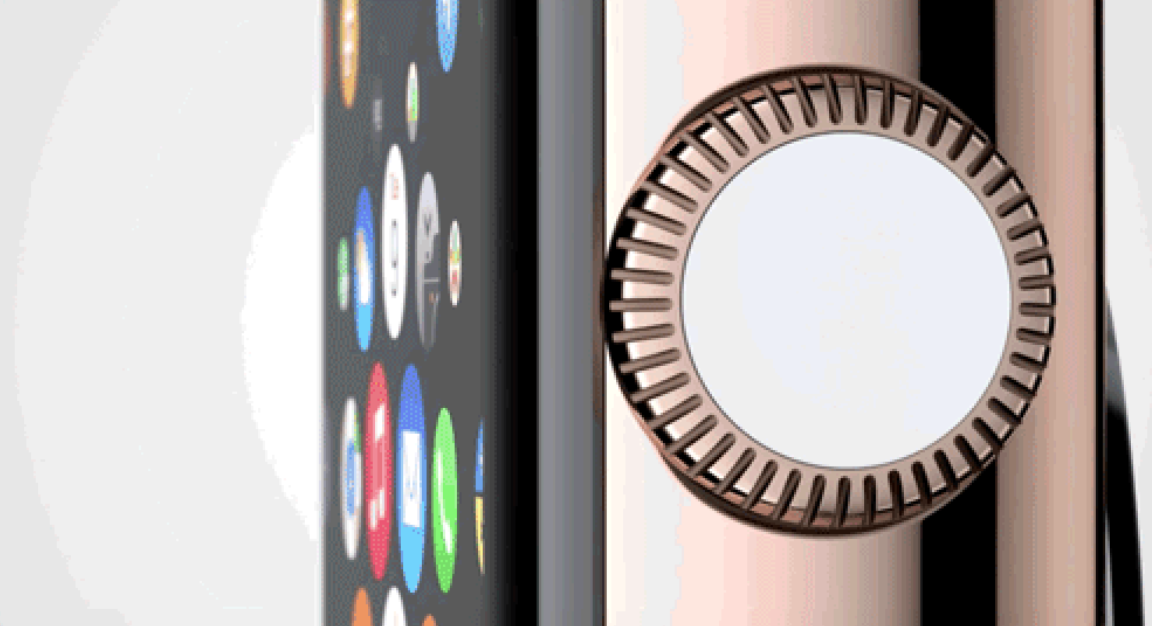
\includegraphics[scale=0.5]{applecrown}

The Apple Watch interface itself is well-known, a touch screen with apps that users can press. If the user is already an owner of an iPhone, then the mental model is even more intuitive for them. Force Touch is a new addition to the Apple brand however, and the mental model seems to have a disconnect for the inexperienced users. Force Touch is supposed to make the user experience smoother, faster, and more intuitive. From the developer's side, the user can open a new text message quickly from the messages app,  change the face of their watch, or stop directions, all done quickly using Force Touch. However, many people were either not aware of Force Touch, or weren't sure what it would do or when it could be used. This is because we are not familiar with technologies, especially delicate ones, that need to have pressure as a source for extra functionality. When these devices cost hundreds of dollars, people tend to be careful with them, scared to break or damage the devices. There is, in my opinion, a whole new world for dynamic interaction which can allow the user to be incredibly efficient, but it will have a moderate learning curve. \par

Google Glass is a much more ambitious and difficult product to attempt to make. There was never a product that was in it's first iteration with no predecessors that did something perfectly. Google took on a difficult challenge, and tried to add a HUD display with a touchpad to glasses. The developer's mental model appears to be simple, have the user flick the touchpad or tilt their head up and have Google Glass do something, such as directions, take a photo, etc. In theory, if it was optimally designed, it would prove to be more efficient than Apple Watch, since the user can just continue walking without having to look down at a screen. The user slides back or forth on the pad to cycle through menus, tapping to make a selection, and can hold down to do a search without the voice command. \par

\par In practice, the interface is not intuitive for new users, they reported the device to be uncomfortable with long load times. 3 out of 10 users reported the device got too hot to wear, and wanted to take it off. One user wanted a color blind mode, while 4 out of 10 wanted a tutorial on how to use the maps function. Another user wanted to switch the lens from the right eye to the left eye. \par
 As for the Apple Watch testers, they too wanted some tutorials on how to use the maps, but overall thought it was a useful gadget once one learned how to use it. One user said it could use some speed tweaks, and that albeit the device being "cool", he would rather stick with his normal watch and use his phone. A reviewer for the Apple Watch found that instead of minimizing time on his phone or watch, he found himself looking at it more frequently. He would get messages and alerts, and was even asked if he had some place to be during a meeting. \par
 
 To conclude, the Apple Watch seems to have better interaction design implementations based on our data, scoring far greater in efficiency, having less errors than Google Watch, and higher user satisfaction. 


\newpage

\begin{center}
Sources
\end{center}
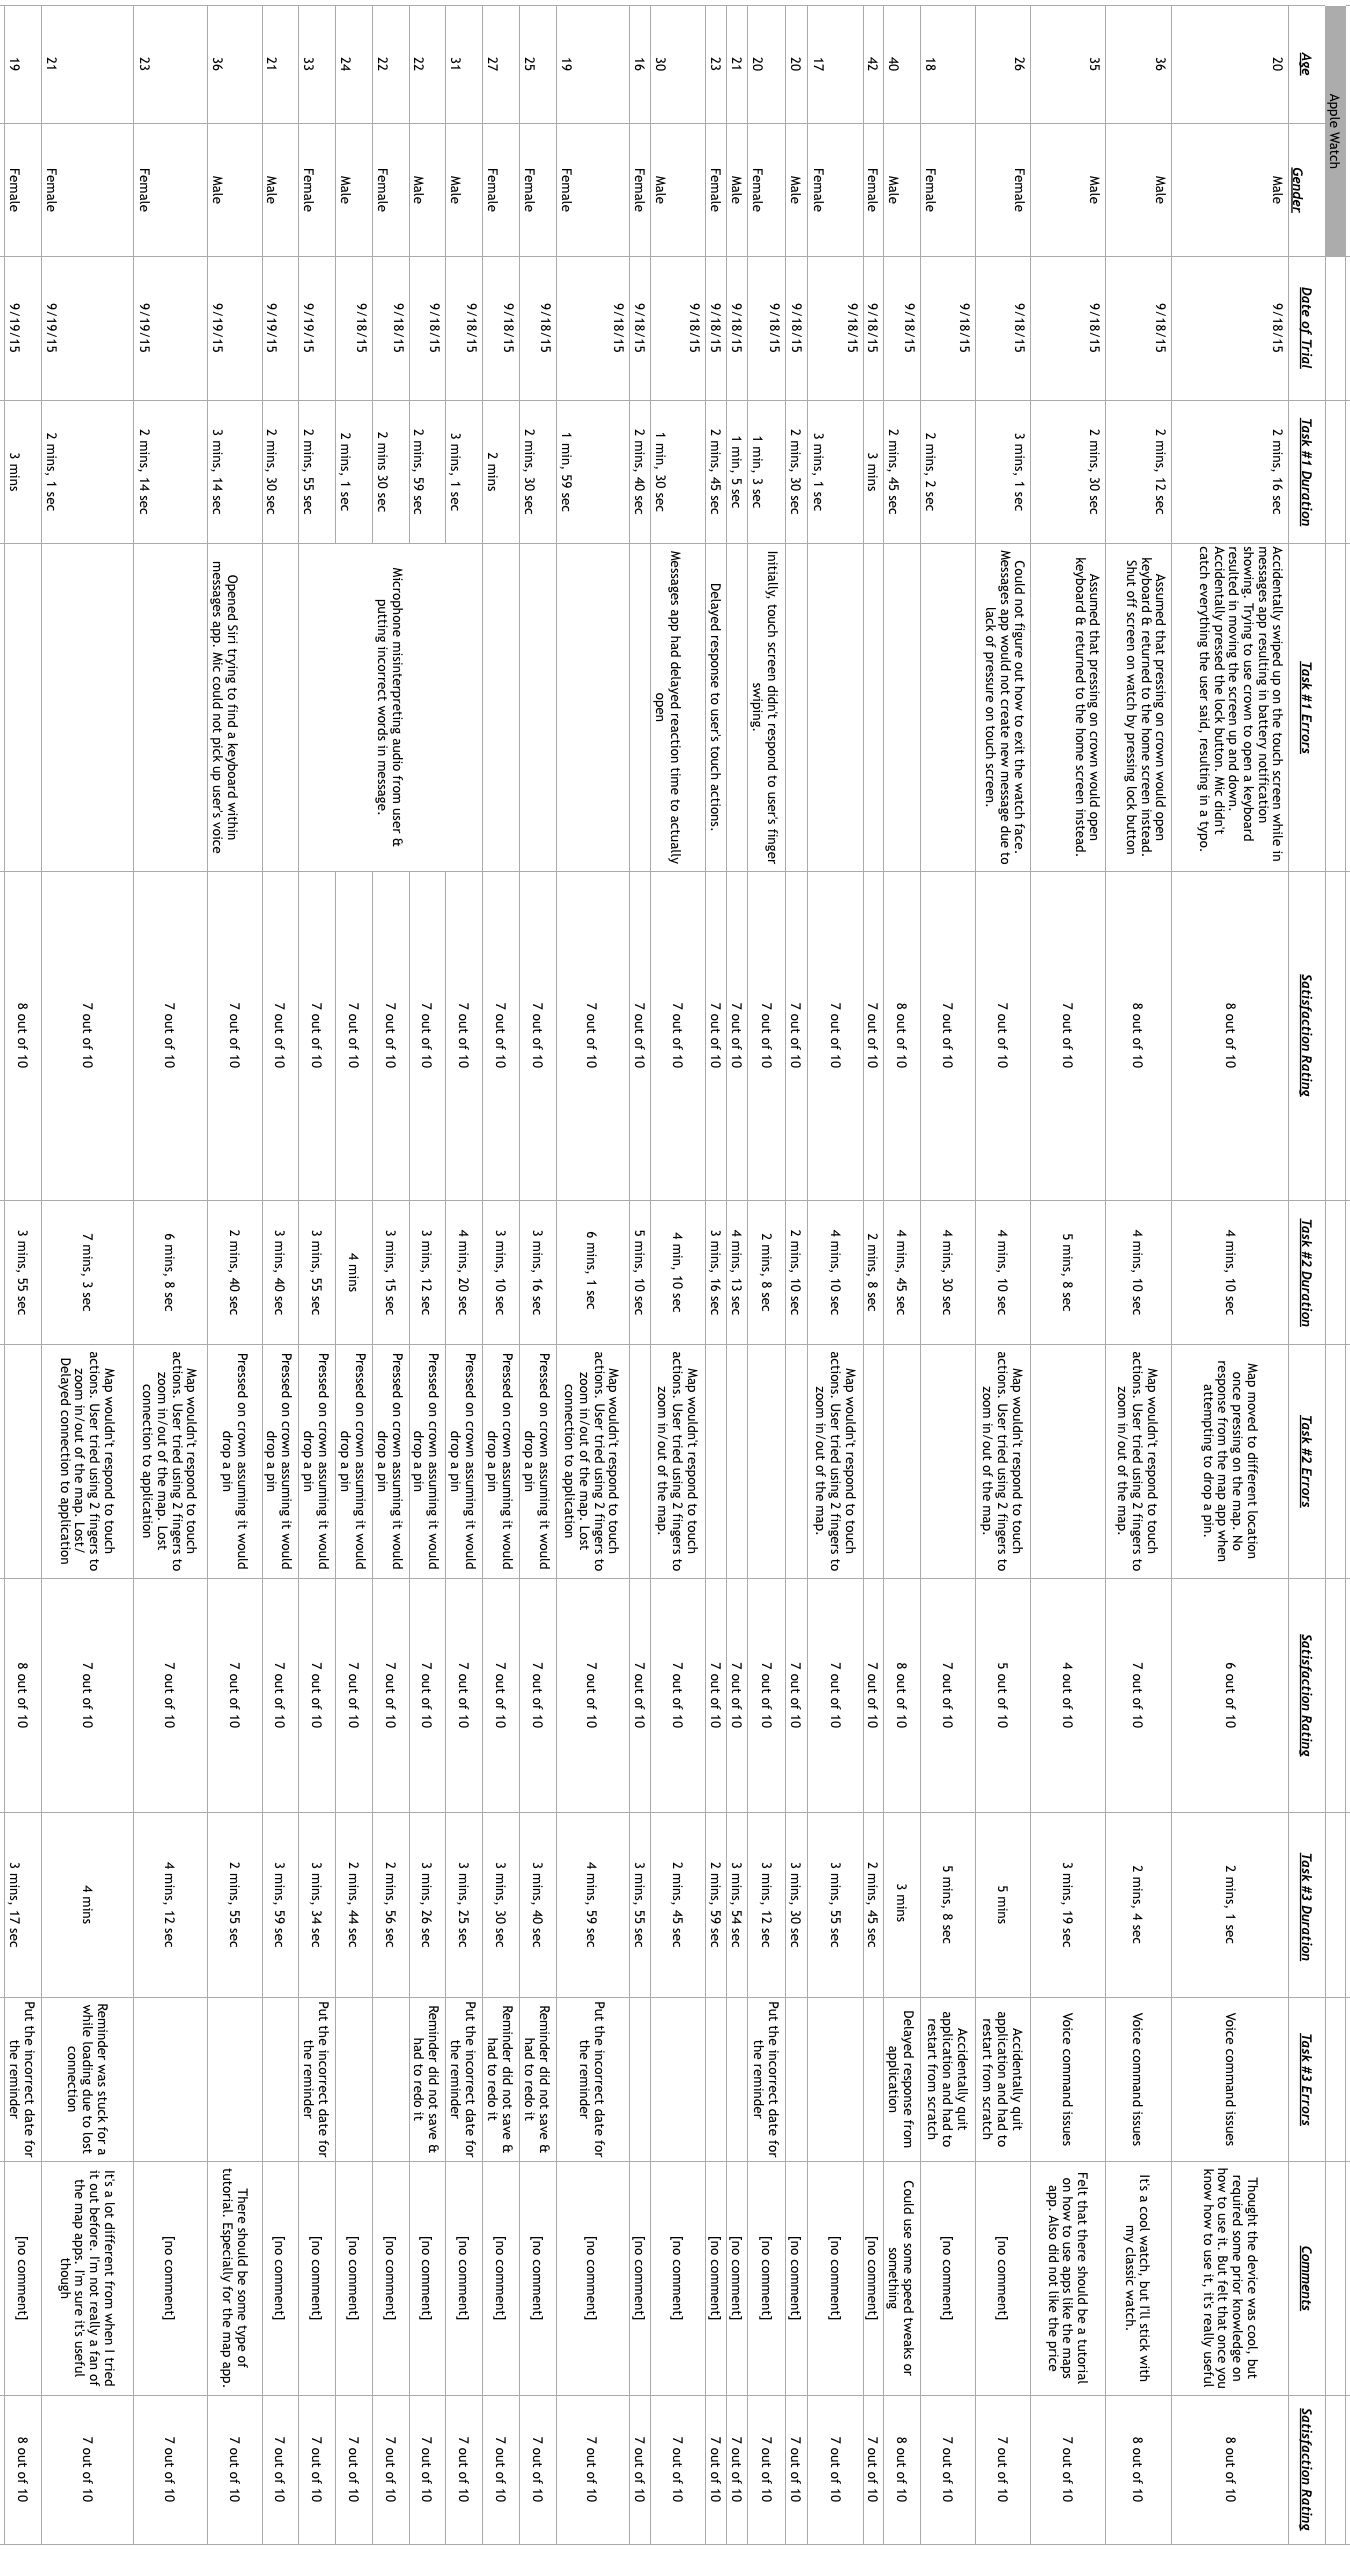
\includegraphics[scale=0.45]{sources1}
\newpage
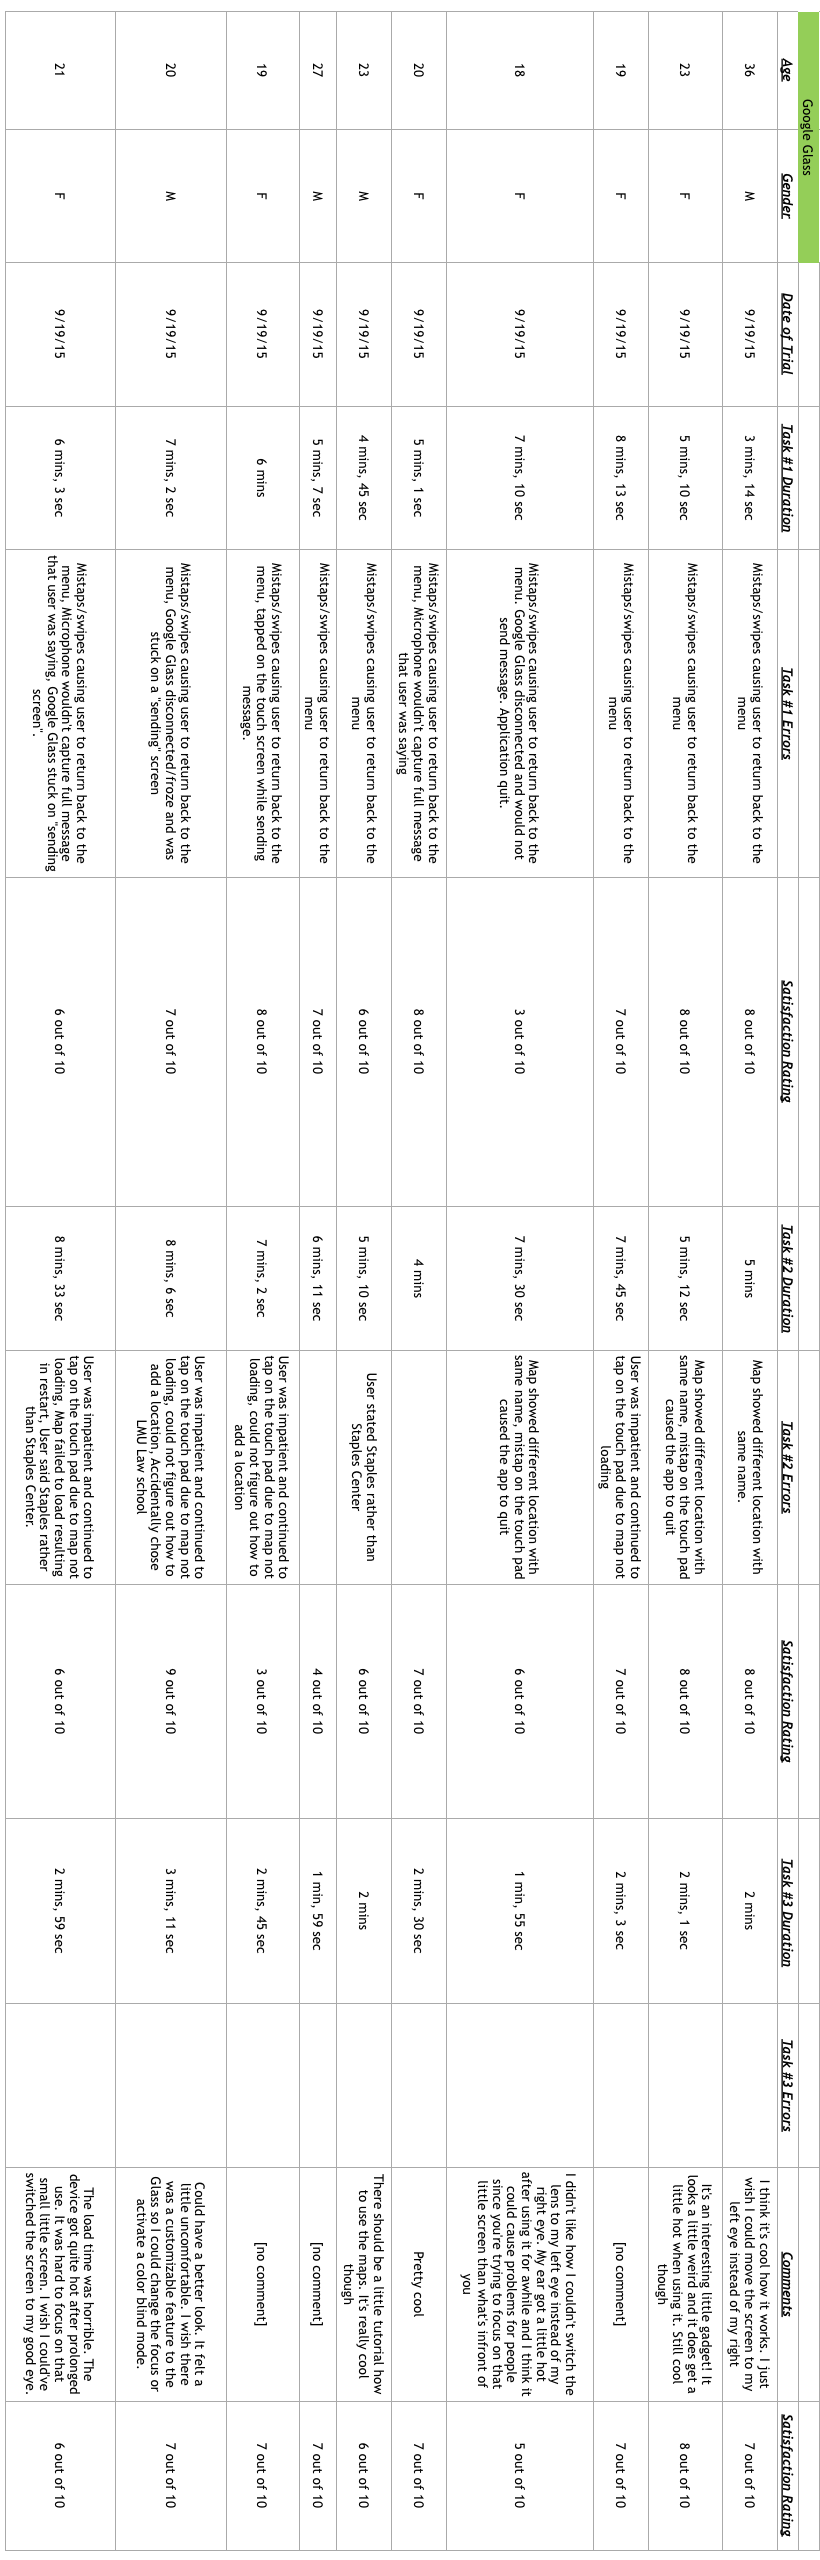
\includegraphics[scale=0.45]{sources2}

\newpage
Kaipa, Prasad. "Ivey Business Journal." Ivey Business Journal. N.p., n.d. Web. 24 Sept. 2015.\\

Polaine, Andy. "The Apple Watch, Skeuomorphism and Metaphors." Polaine.com. N.p., 25 Mar. 2015. Web. 24 Sept. 2015.\\

Apple Inc. "Design Principles." Apple.com. Apple, 04 Aug. 2015. Web. 24 Sept. 2015.


\end{document}